\chapter{Perancangan}
\label{perancangan} 

\section{Struktur Proyek Moodle Mobile}

Proyek Moodle Mobile terdiri dari kumpulan file-file dan direktori-direktori utama yang mengandung fungsi dan \textit{source code} untuk aplikasi Moodle Mobile, platform Android dan iOS, alat untuk mebangun perangkat lunak, dan konfigurasi. Struktur dapat dilihat pada Gambar \ref{fig:project-directory}.
\begin{figure} [H]
	\centering  
	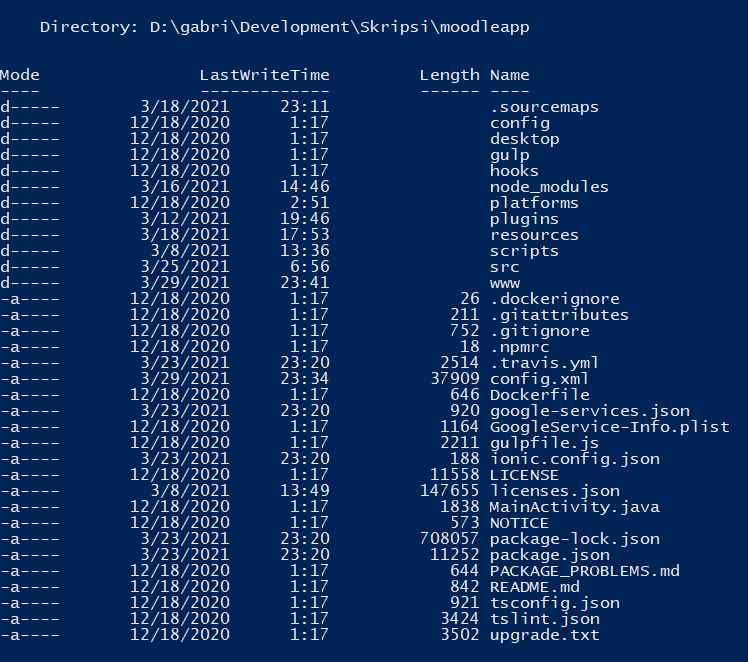
\includegraphics[scale=0.5]{project-directory.PNG}  
	\caption[Struktur direktori proyek Moodle Mobile] {Struktur direktori proyek Moodle Mobile}
	\label{fig:project-directory} 
\end{figure}  

Perubahan pada proyek akan sering dilakukan pada direktori \texttt{src}, dan \texttt{config.xml}. Direktori \texttt{src} berisi kode-kode utama dari aplikasi Moodle mobile dan konfigurasinya. Konfigurasi dari Moodle mobile sendiri diatur oleh file \texttt{config.json} di dalam folder \texttt{src}. File \texttt{Config.xml} berfungsi untuk mengatur konfigurasi dari aplikasi Cordova. Dikarenakan Moodle mobile menggunakan Cordova maka pengaturan saat melakukan \textit{build} untuk perangkat bergerak akan diambil dari file \texttt{Config.xml}. 